% 2013 全国卷Ⅰ文科第 19 题：三棱柱 ABC-A_1B_1C_1，虚线为隐藏棱。
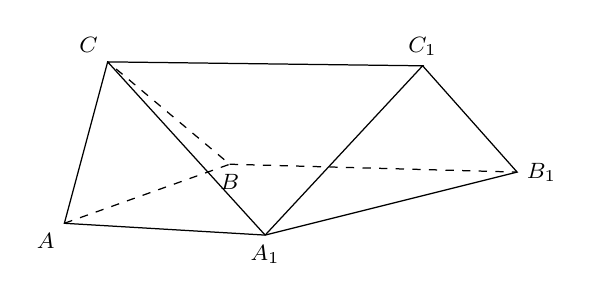
\begin{tikzpicture}[font=\footnotesize, line width=0.45pt]
  \coordinate (A) at (0,0);
  \coordinate (C) at (0.55,2.05);
  \coordinate (B) at (2.10,0.75);
  \coordinate (A1) at (2.55,-0.15);
  \coordinate (C1) at (4.55,2.00);
  \coordinate (B1) at (5.75,0.65);
  \draw (A)--(C)--(C1)--(A1)--cycle;
  \draw (C1)--(B1)--(A1);
  \draw (C)--(A1);
  \draw[dashed] (A)--(B)--(C) (B)--(B1);
  \node[below left] at (A) {$A$};
  \node[above left] at (C) {$C$};
  \node[below] at (B) {$B$};
  \node[below] at (A1) {$A_1$};
  \node[above] at (C1) {$C_1$};
  \node[right] at (B1) {$B_1$};
\end{tikzpicture}
